\section{VECSEL basics}
\label{sec:basics}

In this section
I introduce the concepts
relevant to understand
the presented measurements.
The topic of VECSEL
is rich and diverse:
for more extensive reviews
I direct to
Tropper et al. \cite{Tropper2006}
and Calvez et al. \cite{Calvez2009}.

\subsection{Structure and design choices}

VECSEL
stands for
vertical-external-cavity
surface-emitting
laser.
They
are composed of
three main sections:
the confinement window,
the gain region,
and the active mirror.
This mirror,
together with
an external output coupling mirror,
form the laser cavity;
thus the name.
VECSELs are usually
optically pumped.
One of the characteristics
of VECSELs
is their ability
to convert low quality pump
to high quality emission light.
The incidence angle
is chosen to be convenient
for the setup at hand \cite{Tropper2006},
but should not be too flat,
in order to limit
the pump spot to elongate.
Figure~\ref{img:vecsel_principle}
illustrates the basic elements.

\begin{figure}
\centering
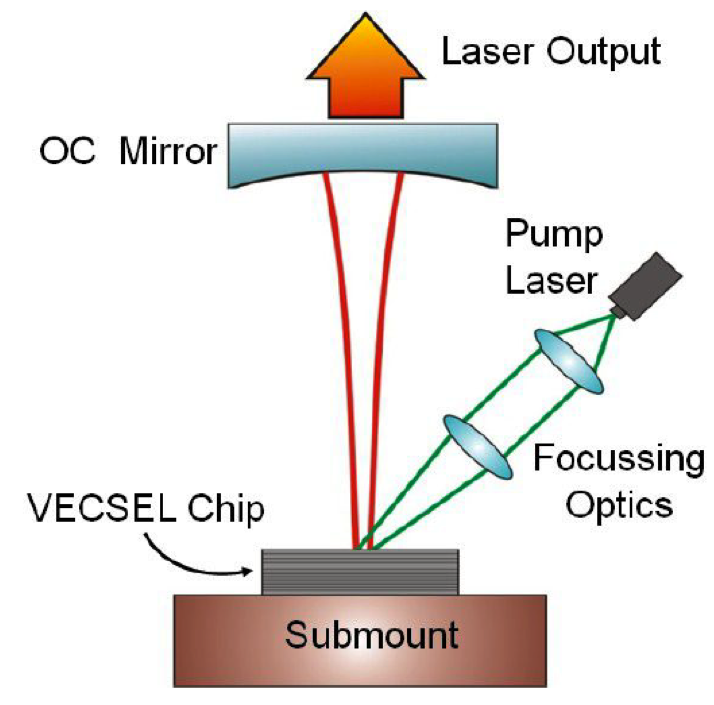
\includegraphics[width=10cm]{img/vecsel_principle.png}
\caption{An optically pumped
vertical-external-cavity
surface-emitting laser
(VECSEL)
is composed of
an output coupler
external mirror (OC)
and the VECSEL chip itself.
The VECSEL chip is composed of
a window layer
(also known as cap),
a gain region,
and a mirror.
It is mounted
on a heat sink,
and pumped
by a diode laser.
From \cite{Sirbu2014SPIE}.}
\label{img:vecsel_principle}
\end{figure}

The active mirror
is composed of
a periodic structure
of quarter wavelength
semiconductor layers;
a distributed Bragg reflector (DBR).
The materials used for the DBR
have to fulfill
three basic requirements
\cite{Calvez2009}.
First of all,
the material has to be transparent,
i.e. non-absorbent,
at the emission wavelength.
Secondly,
the used materials
have to have a high contrast
of refractive index.
This helps to obtain
high reflectivity
with a low number of layers;
smaller devices
have advantageous thermal properties.
Thirdly,
the material used
has to be as thermally conductive as possible.

The gain region
is composed of
quantum wells (QWs).
They are placed
at the antinodes
of the standing-wave
of the optical field
of the design wavelength.
This so-called
resonant periodic gain (RPG)
configuration
helps to avoid spatial hole burning
\cite{Ranta2014OptLett}.
Figure~\ref{img:design}
illustrates our VECSEL chip.

\begin{figure}
\centering
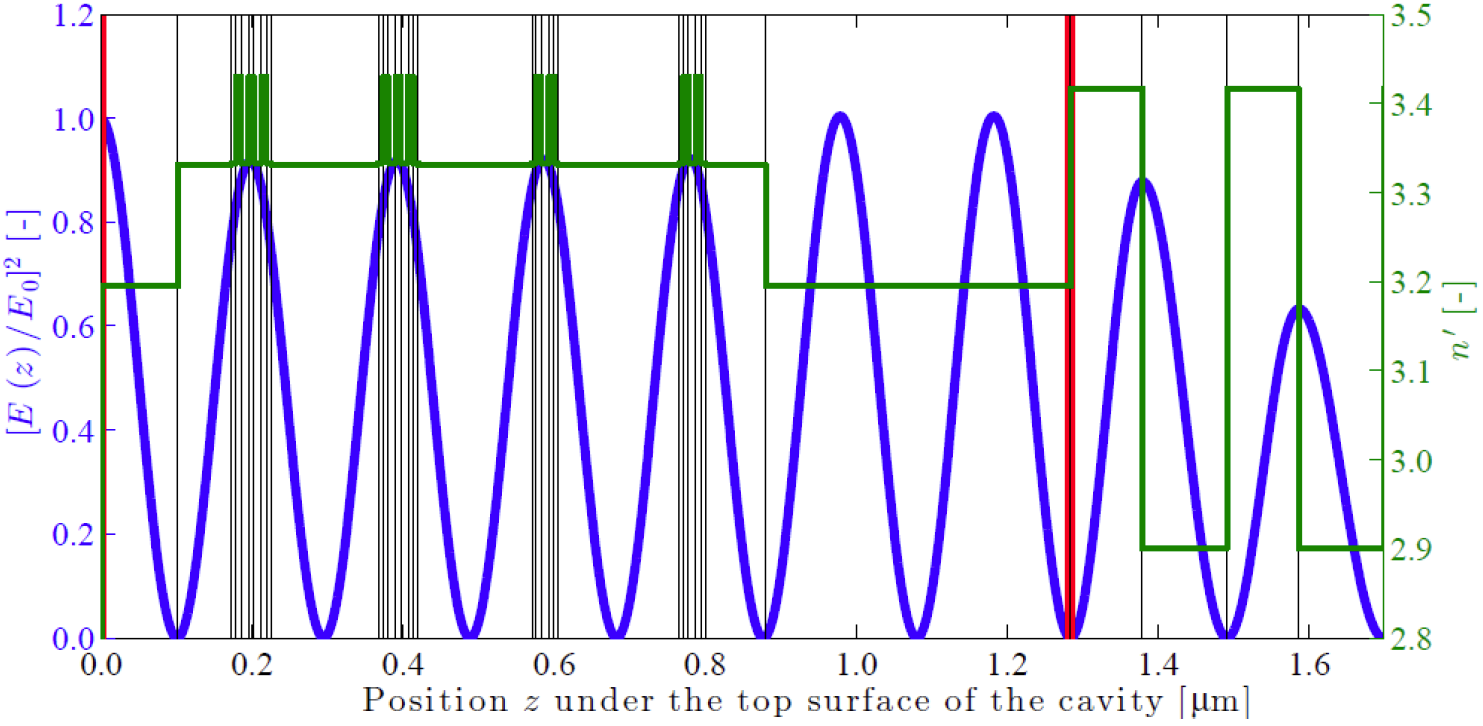
\includegraphics[width=14.5cm]{img/design.png}
\caption{Schematic depiction of our VECSEL structure,
from \cite{Sirbu2014SPIE}.
The first layer from left
is the confinement window
(also known as cap).
It is followed by the
gain region,
up to the red line.
This line indicates
the wafer-fusion interface,
after which follows the DBR.
Only the first two layer pairs
of the DBR
are shown;
there are 24 over all.}
\label{img:design}
\end{figure}

The confinement window
(also known as cap)
is transparent for
pump and signal.
Its function is twofold
\cite{Tropper2006,Calvez2009}.
First,
it is designed to provide
good coupling between
the external and
the sub-cavity.
Secondly,
it is a spacer
to separate the surface
from the carriers
generated in the active region.
This reduces non-radiative recombinations.

The thermal management
is critical for the operation
of VECSELs.
Over the years,
two strategies
for heat extraction
have been established
\cite{Kemp2008,Vetter2012}:
the heat-spreader,
and the thin-disk approach.
In the first strategy
the VECSEL chip is grown
in the order
DBR--gain--cap,
and the heat is extracted
through a chemical vapor deposited
(CVD) diamond
clamped onto the cap.
In the second approach,
the structure is grown
in reverse order,
so the Bragg mirror
can be bonded
onto a CVD diamond.
In this strategy
the heat has to be extracted
through the whole structure.

The heat-spreader approach
tends to be more efficient
to extract the heat --
at least
for relatively small pump spot sizes
\cite{Vetter2012}.
On the down side,
it introduces Fabry-Perot effects,
and makes the device packaging
more bulky over all.
For these reasons
the thin disk approach
would be preferred
for a wide variety
of applications \cite{Ranta2014OptLett}.

\subsection{Wafer-fusion}

With our VECSEL design
we aim to cover
the $1.3\,\mu\mathrm{m}$
wavelength band.
The corresponding material system
for the active region
is InP.
DBRs grown on this material system
do not provide high contrast
in refractive index
and have very low thermal conductivity.
Because of the low contrast,
more layers
are required
in order to obtain
high reflectivity.
And this is unfortunate
for the thermal management,
further aggravated by the low conductivity.
Consequentially,
the highest output powers
in this waveband
were obtained for wafer-fused
devices \cite{Ranta2014OptLett}.
For wafer fusion
the active region
is grown separately
from the DBR
and in a second step
fused along the interface
indicated in Fig.~\ref{img:design}
with red line.

This approach corresponds to
the thin disk strategy
mentioned above.
But it has the additional advantage
to combine material systems
whose design wavelength
is around $1.3\,\mu\mathrm{m}$,
with GaAs-based DBR,
whose contrast in refractive index
and thermal conductivity
allows a more efficient heat extraction.
This property is key
for the high power performance
of wafer-fused devices.
Figure~\ref{img:wafer_fusion}
shows a schematic illustration
of our wafer-fused design.
The DBR is bonded
onto the CVD diamond
using a gold interface.
The DBR-Au bond itself
is realized by employing
titanium as adhesion layer.

Alternatives for
the Au-Au-bonding
involve intermediate In solder.
But this material choice
is disadvantageous
for high temperatures
\cite{Ranta2014OptLett}.
Beside the structural necessities
to use the gold layer,
it is also predicted
to show benefits
for the thermal behavior
and conversion efficiency
of a VECSEL
\cite{Hader2011,Devautour2013}.

The design and
manufacturing process
of the samples
was not within the scope
of this project.
I thus constrain myself
to explain only
the essentials
of these processes
necessary
to understand the report
at hand.
A more detailed description
of the manufacturing process
is given in \cite{Ranta2014OptLett,Sirbu2014SPIE}.

\begin{figure}
\centering
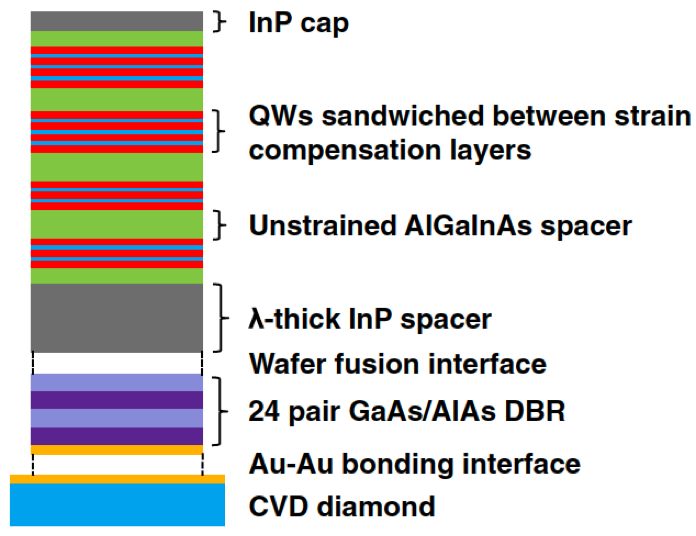
\includegraphics[width=8cm]{img/wafer_fusion.png}
\caption{Our InP-based VECSEL design
incorporating AlGaInAs quantum wells (QWs),
wafer-fused,
and bonded on CVD diamond.
The $\lambda$-thick InP spacer
acts as a defect blocking layer.
The gain region was grown
by metallorganic vapor phase epitaxy (MOVPE),
the DBR was grown
by molecular beam epitaxy (MBE).
From \cite{Ranta2014OptLett,Sirbu2014SPIE}.}
\label{img:wafer_fusion}
\end{figure}
